\documentclass[twocolumn, letterpaper]{scrartcl}

\usepackage{uog_factsheet}
\usepackage{xcolor}
\usepackage{hyperref}

\definecolor{seablue}{RGB}{0,127,169}

\begin{document}
    \title{\color{seablue}User Consent \& Privacy Policies Project}

	\maketitle
	
    % \section*{Instructions}
    
    % \begin{itemize}
    %     \item Open history of your browser, choose 3 websites from your browsing history, open these 3 website in a private/incognito window
    %     \item Is there a consent banner? Does it comply with elements of valid consent (Free, specific, informed, unambiguous)?
    %     \item Check the slides to validate your analysis, write a 2-page report with your analysis.
    % \end{itemize}
    
    \section*{Website Choices}
        
         For the sake of diversity of industries, three websites were selected: \textbf{Games Workshop}\cite{GW} (the world's miniatures game retailer, see Fig. \ref{fig:a}), \textbf{Le Monde}\cite{LM} (A French newspaper, see Fig. \ref{fig:c}) and \textbf{LinkedIn}\cite{LD} (the largest professional social media in the world, see Fig. \ref{fig:d}).
	
	\section{Analyses of the websites' policies and consent-handling}
	
	    We recall that consent forms are a mechanism to give data subjects control and choice over whether or not their personal data will be processed. It must be given before any processing starts and is only valid when four elements of valid consent (based on the General Data Protection Regulation's article 4(11)) are met: i) \textbf{Free}, ii) \textbf{Specific}, iii) \textbf{Informed}, iv) \textbf{Unambiguous}.
	
    \subsection*{Games Workshop's}

	    Games Workshop's cookie policies provides an \textbf{example of a consent policy regarding the use of cookies on their website that is not free, specific, informed or unambiguous}.
	
    	\textbf{The consent policy is not free}. The data subject has no real choice when presented with the consent banner, which is more of a warning than a prompt: "\textit{This website uses cookies to personalise content and advertising, and to analyse our traffic. By continuing to use this site you are agreeing to our use of cookies}". We could qualify this instance as an \textit{imbalance of power} as there is coercion involved -- the data subject has no choice but to click the \textit{continue} button. We also see that \textit{conditionality} and \textit{detrimentality} are involved (See Fig. \ref{fig:b}). Indeed, if the data subject personally sets up their browser to restrict cookies, they may suffer a loss in functionality on the website \footnote{It must be noted that Games Workshop provides no possible way to restrict the use of cookies on their website. They explicitly mention that the data subject should actively parameter their browser via the use plug-ins or processes described off-website by unrelated third-parties -- see Fig. \ref{fig:b}.}.
    	
    	\textbf{The consent policy is not specific}. The purpose is \textit{too wide to be specific}, mentioning cookies would be used "to personalise content and advertising, and to analyse our traffic" in the main page banner. Further detail is provided in their Cookie Notice page\cite{GW_CN} but with a lack of choices provided to the data subject, \textit{the website proves itself to not provide any granularity in consent requests}. The same remark can be done with regards to an absent clear separation of consent request depending on the requested information and later use for it. 
    	
    	\textbf{The consent policy does not allow informed consent}. The language and instructions for people to opt out of tracking are not meant for lay people as shown in Footnote 1. Similarly the type of data to be collected and shared is not present in the Cookie Notice page -- the right to withdraw consent (as per GDPR Article 7(3)) does not exist.
    	
    	\textbf{The consent banner presents an example of ambiguous consent}. The only possible action is to "continue" and close the cookie banner.
    	
    	In conclusion, Games Workshop has a poor implementation of a user consent and privacy policy with regards to GDPR, failing to meet all four criteria of a valid consent as per GDPR's Article 4(11). A point of note is that the Cookie Notice page mentions that the website uses a technology called Web Beacon, which is not fully stated in the consent bar on the front page and which cannot be opted-out as with the rest.
 	
 		\begin{figure}
    % 		Figure 1\label{fig:a}. Games Workshop's Main Page
    		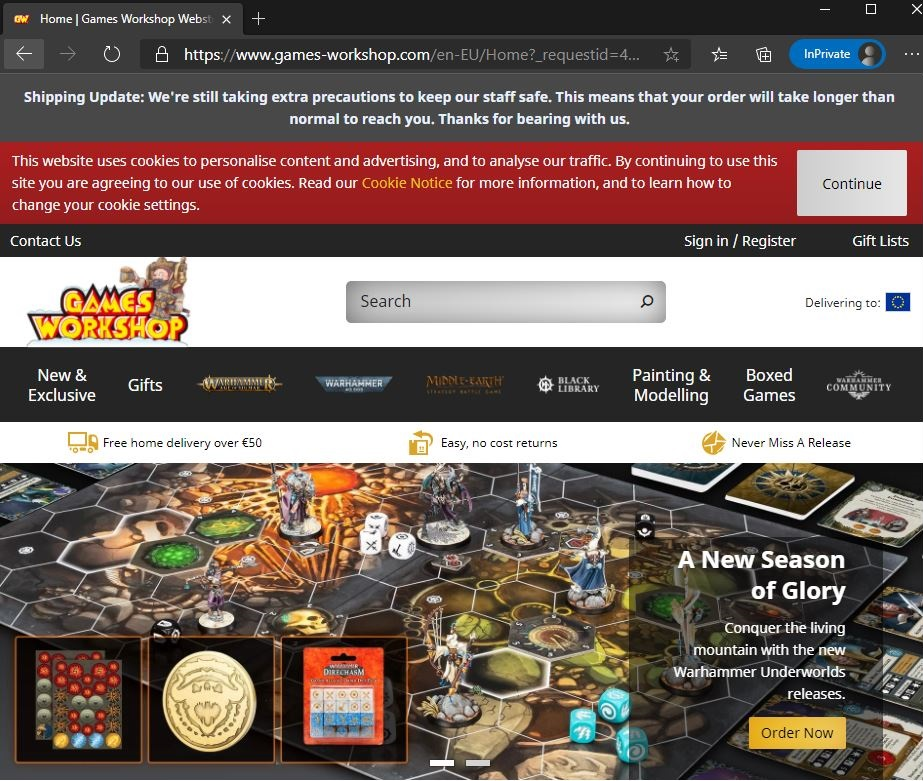
\includegraphics[width=0.95\linewidth]{gw_website.JPG}
     		\caption{Games Workshop's Main Page \label{fig:a}}
     	\end{figure}
    
        \begin{figure}[tbp]	
            % Figure 2\label{fig:b}. Example of conditionality in Games Workshop's policy
            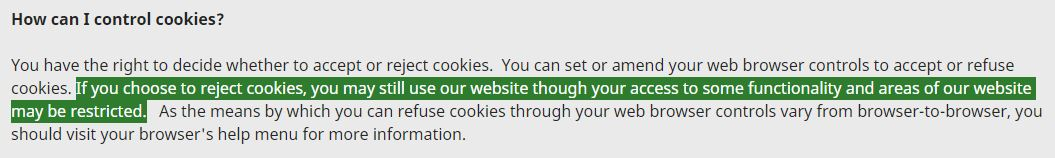
\includegraphics[width=0.95\linewidth]{conditionality.JPG}
            \caption{Example of conditionality in Games Workshop's policy \label{fig:b}}
        \end{figure}
        
	\subsection*{Le Monde's}

    	Le Monde's website provides elements that would confirm that consent given by data subjects is \textbf{free}, \textbf{specific}, \textbf{informed}, and \textbf{unambiguous}. However, we will present two caveats that would put the free and informed aspects of it into questions. 
        
    	OVerall, there is no presumption of imbalance of power, and consent is clearly asked in the scope of providing news content to the data subjects. Specific consent is present as the purpose is specified and there is available granularity for the data subjects to selectively opt-in to cookie tracking (e.g. When personalizing the cookie policy, the tracking options are ticked off by default. The possibility to refuse all cookies, besides those legally-allowed to be non-opt-out, is available -- See Fig. \ref{fig:d}). Finally, the consent can be qualified as informed as the purpose of the processing is started on the front page (See Fig. \ref{fig:c}) while the type of data to be collected and shared with third parties is detailed in the parameter page. the overall intent of Le Monde with the data is unambiguous.
    	
    	\begin{figure}[tbp]	
            % Figure 3\label{fig:c}. Le Monde's Main Page 
            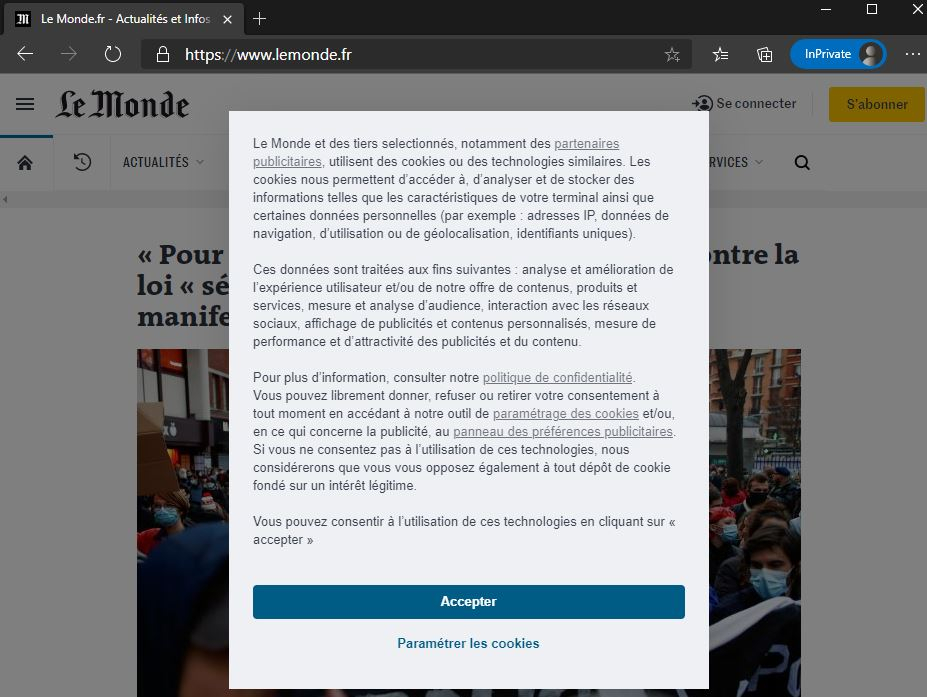
\includegraphics[width=0.9\linewidth]{lm_website.JPG}
            \caption{Le Monde's Main Page \label{fig:c}}
        \end{figure}
        
    	However, one possible criticism that might put into question the validity of the data subjects' consent is that, were they to refuse all cookies, Le Monde's website would display a irremovable advertisement for their subscription service, which can be obstructing on some devices (See Fig. \ref{fig:e}). \textbf{This could unmake the argument that Le Monde's policy fulfills the 'free' criterion of valid consent as stated by Article 4(11) of GDPR}. This irremovable ad bar could be considered a detriment and a consequence of not consenting. On the other hand, there is no prior indication that this bar would appear if the cookies were kept deactivated. This bar is not used as a threat to the data subjects' experience on the website. It might only be an issue only on some types of devices for which the website was not optimized for (e.g. small-screen-factor devices). 
    	
    	\begin{figure}[tbp]
            % Figure 4\label{fig:d}. Le Monde's Cookie Policy Parameter Page 
            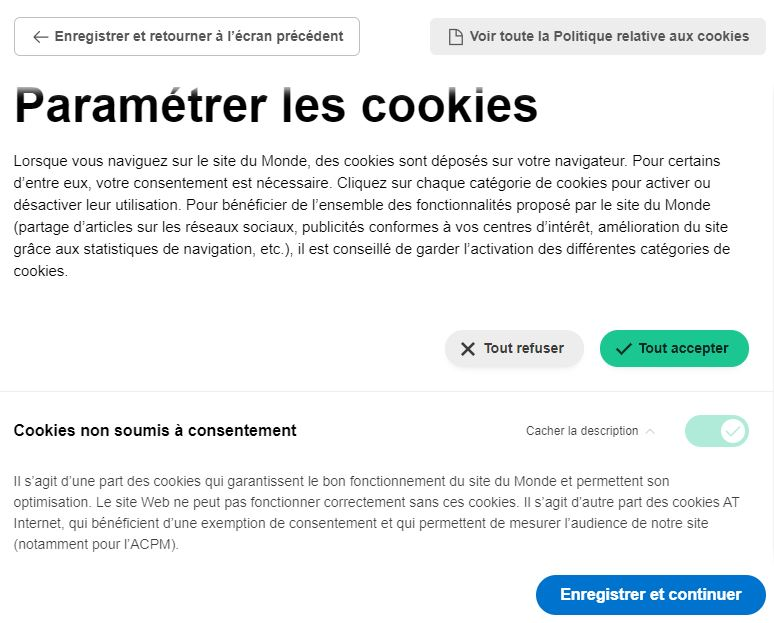
\includegraphics[width=0.9\linewidth]{lm_cn.JPG}
            \caption{Le Monde's Cookie Policy Parameter Page \label{fig:d}}
        \end{figure}
        
    	Another criticism would be accessing the detailed Cookies and Privacy Policy page\cite{LM2}, which happens to be \textbf{unreadable if the data subjects have not yet accepted the policy}, i.e. there is no way for a data subject to read the detailed policy (which does include a table dedicated to describing the type of cookies used by Le Monde, the data collected and shared, and a purpose and expiration date associated to each) without accepting the cookies first (See Fig. \ref{fig:f}). This implies that there couldn't possibly be an informed consent with regards to the cookie policy on Le Monde's website. Recital\$42 and Article 7(3) of GDPR might not be fully satisfied. 
        
        \begin{figure}[tbp]
            % Figure 5\label{fig:e}. Le Monde's Unremovable Ad Bar
            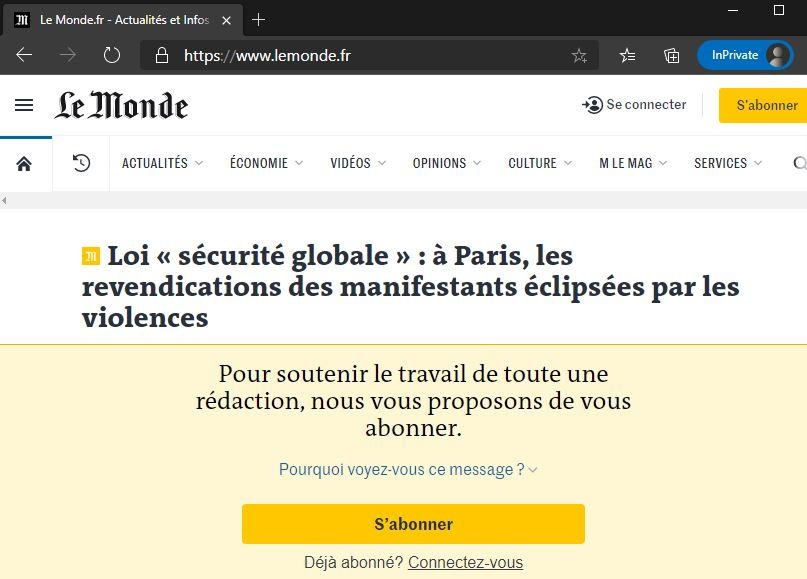
\includegraphics[width=0.95\linewidth]{lm_sub.JPG}
            \caption{Le Monde's Unremovable Ad \label{fig:e}}
        \end{figure}
        
        \begin{figure}[tbp]	
            % Figure 6\label{fig:f}. Le Monde's Unreadable Detailed Cookie Policy
            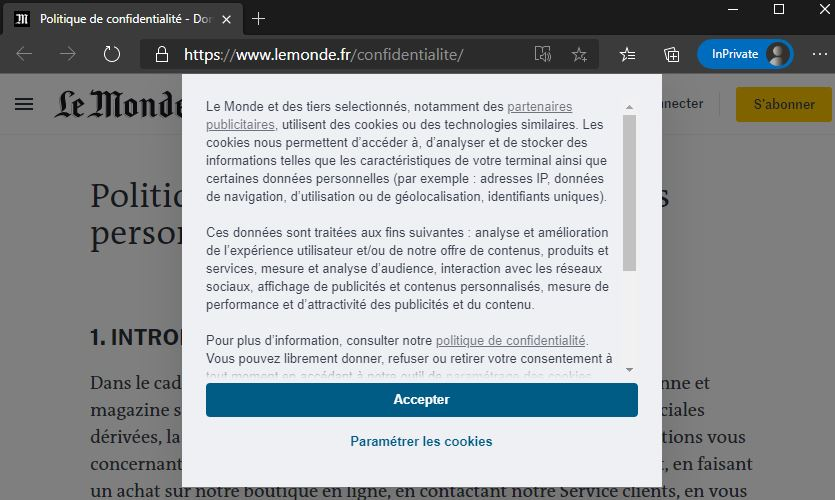
\includegraphics[width=0.95\linewidth]{lm_policy.JPG}
            \caption{Le Monde's Unreadable Detailed Cookie Policy\label{fig:f}}
        \end{figure}
        
        \begin{figure}[tbp]	
        % Figure 6\label{fig:g}. LinkedIn's Main Page 
        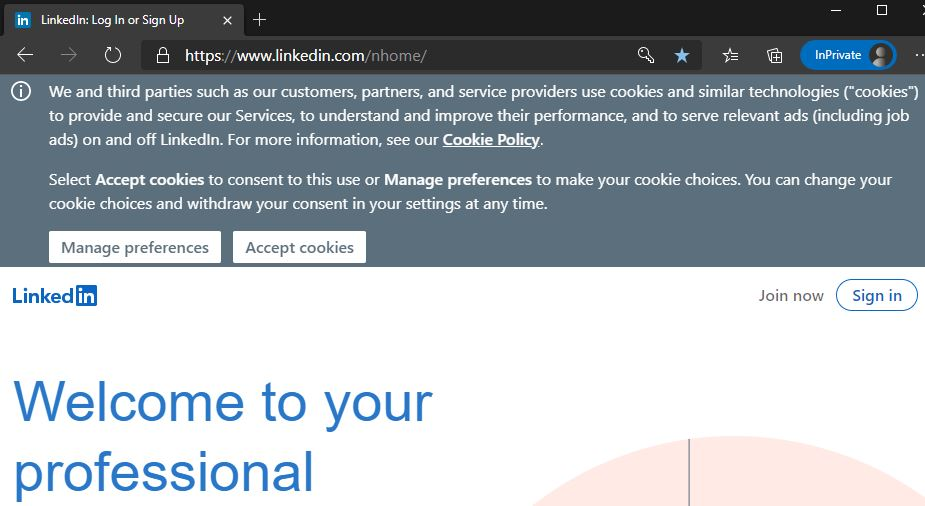
\includegraphics[width=0.95\linewidth]{ld_website.JPG}
        \caption{LinkedIn's Main Page \label{fig:g}}
        \end{figure}
        
	\subsection*{LinkedIn's}
	    
	    Similar to Le Monde's website, LinkedIn provides elements proving that consent given by data subjects is \textbf{free}, \textbf{specific}, \textbf{informed}, and \textbf{unambiguous}. For instance, LinkedIn provides a detailed Consent Bar (See Fig. \ref{fig:g}) as well as a dedicated cookie page where data subjects can decide to opt-in (See Fig. \ref{fig:h}).
        
	    As with Le Monde, LinkedIn does provide a [more] detailed Cookie Policy page that contains a table dedicated to describing the type of cookies used, the data collected and shared, and a purpose and expiration date associated to each. LinkedIn happens to not hide that page behind a pop-up page.
	    
	    LinkedIn's downside is that, were the data subjects leaving the cookie policy parameter page without inputing any modification (See Fig. \ref{fig:h}), the consent bar would never appear again. I.e. once the cookie parameters have been opened, they are considered set modified and accepted by the data subjects. It is quite user-unfriendly to find that page again in the website's options. This implies \textbf{withdrawal of consent} can be hard to perform.

        \begin{figure}[tbp]	
        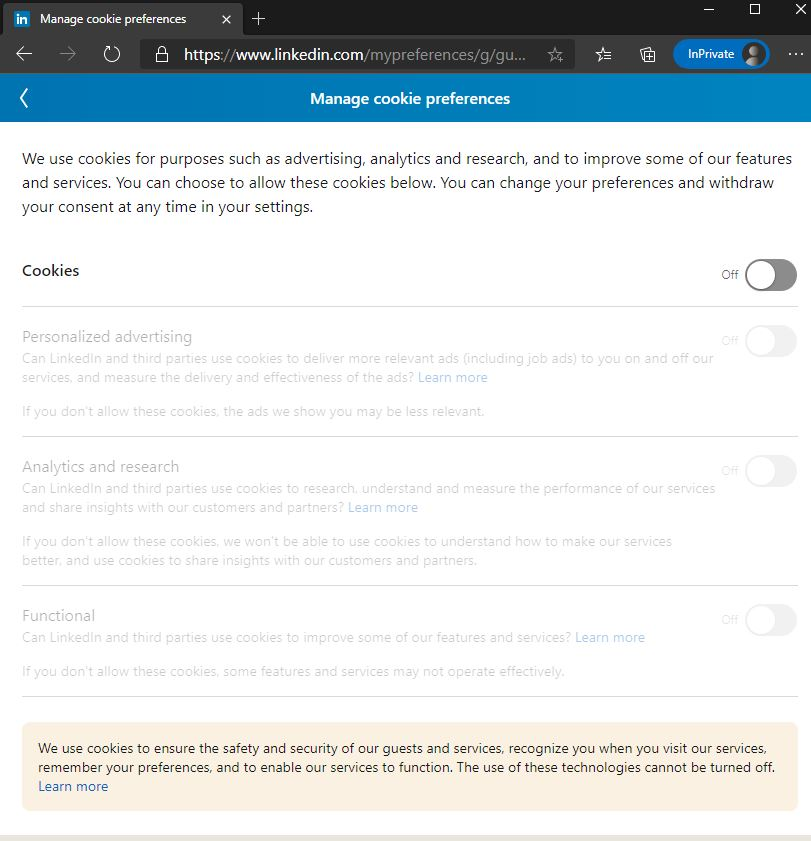
\includegraphics[width=0.9\linewidth]{ld_cn.JPG}
        \caption{LinkedIn's Cookie Policy Parameter Page \label{fig:h}}
        \end{figure}
        
        \begin{figure}[tbp]	
        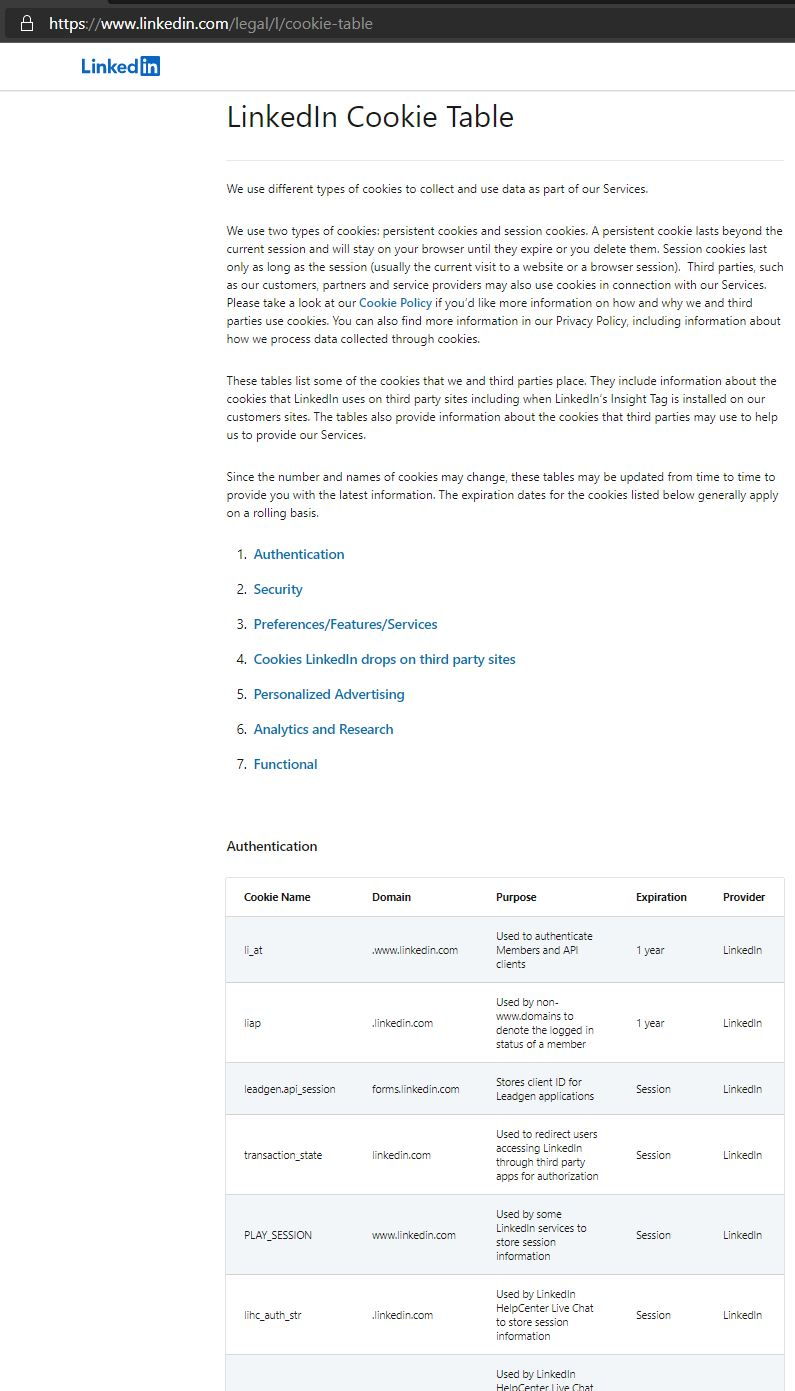
\includegraphics[width=0.9\linewidth]{ld_table.JPG}
        \caption{LinkedIn's Cookie Detailed Policy Page \label{fig:i}}
        \end{figure}
        
	\subsection*{Conclusion}
	
	Out of all three websites, Games Workshop's is the most at fault in how it handles consent from data subjects. It fails in all four categories of validity set by the Article 4(11) of GDPR.
	
	Le Monde and LinkedIn's websites are much more compliant with the article, scoring in all four categories. However, both websites shows failings some cases which means that some doubts can still be cast on the validity of consent on their platforms.
	
    \bibliographystyle{unsrtnat}   
    \begin{thebibliography}{9}

    \bibitem{GW}
    	Games Workshop Limited, \textit{\href{https://www.games-workshop.com/en-US/Home}{website}}.
    	\bibitem{GW_CN}
    	Games Workshop's Cookie Notice page, \textit{\href{https://www.games-workshop.com/en-EU/Cookie-Notice}{website}}.
    \bibitem{LM}
    	Le Monde SA, \textit{\href{https://www.lemonde.fr/}{website}}.
    \bibitem{LM2}
    	Le Monde's Detailed Cookies and Privacy Page, \textit{\href{https://www.lemonde.fr/confidentialite/}{website}}.
    \bibitem{LD}
    	LinkedIn Corporation, \textit{\href{https://www.linkedin.com/}{website}}.

    \end{thebibliography}

\end{document}

